% -*- coding: utf-8; -*-

% Modelo de apresentação da EMC - UFG

% Autor: Pedro Maione [pedromaionee@gmail.com]
% http://github.com/next-ifg/beamer-ufg.git


\documentclass[compress]{beamer}
% --------------------------------------------------------------------------
% Configurações para listagem de código com o pacote Listings
% --------------------------------------------------------------------------
\usepackage{listings}

\lstset{ %
language=[LaTeX]TeX,
basicstyle=\footnotesize\ttfamily,
keywordstyle=,
numbers=left,
numberstyle=\tiny\ttfamily,
stepnumber=1,
showspaces=false,
showstringspaces=false,
showtabs=false,
breaklines=true,
frame=tb,
framerule=0.5pt,
tabsize=4,
framexleftmargin=0.5em,
framexrightmargin=0.5em,
xleftmargin=0.5em,
xrightmargin=0.5em
}



%%% Local Variables:
%%% mode: latex
%%% TeX-master: "ufg-beamer-demo"
%%% End:


% --------------------------------------------------------------------------
% Carrega o tema
% --------------------------------------------------------------------------
\usetheme{ufg}

% --------------------------------------------------------------------------
% General presentation settings
% --------------------------------------------------------------------------
\title{Modelo de Apresentação do Beamer}
\subtitle{Demonstração do modelo do beamer UFG - EMC}
\date{\today}
\author{Nome Sobrenome}
\Orientador{Prof. Furlano de Tal}
\institute{%
  {\bfseries Universidade Federal de Goiás} \\%
  \par%
  Escola de Engenharia Elétrica, Mecânica e da Computação. }

\renewcommand*{\arraystretch}{1.25}

\begin{document}
% --------------------------------------------------------------------------
% Titlepage
% --------------------------------------------------------------------------

\maketitle

% --------------------------------------------------------------------------
% Table of contents
% --------------------------------------------------------------------------
\section*{Sumário}
\begin{frame}
  \frametitle{Sumário}
  \tableofcontents
  % Para não mostrar subsections utilize o comando abaixo
  % \tableofcontents[hideallsubsections]
\end{frame}

% --------------------------------------------------------------------------
% Content
% --------------------------------------------------------------------------
\section<presentation>[Introdução]{Introdução ao Beamer}

\begin{frame}
  \frametitle{Introdução}

  \begin{block}{O que é o \emph{BEAMER}?}
    A classe Beamer para o \ LaTeX \ é utilizada para criar apresentações,
    utilizando um projetor. É gerado um arquivo PDF, podendo ser mostrado com
    grande número de programas.
  \end{block}
  
\end{frame}


\section<presentation>[Exemplos]{Exemplos de utilização}

%% Atenção
%
% Entre uma section e uma subsection deve haver ao menos um frame.
% Utilize o exemplo de frame abaixo com o sumário da subseção

\begin{frame}
  \frametitle{Sumário da Seção}
  \tableofcontents[currentsection]
  \InsereBackgroung %% Insere o background com Logo UFG
\end{frame}

\subsection{Blocos}


\begin{frame}[fragile]
  \frametitle{Blocos}
  \begin{block}{Bloco simples}
    Este é um exemplo de utilização do bloco.
\begin{lstlisting}
\being{block}{Titulo do bloco}
      %% Conteudo
\end{block}
\end{lstlisting}
  \end{block}
\end{frame}


\begin{frame}[fragile]
  \frametitle{Blocos}
  \begin{alertblock}{Bloco Alerta}
    Este é um exemplo de utilização do bloco de alerta.
\begin{lstlisting}
\being{alertblock}{Titulo do bloco}
%% Conteudo
\end{alertblock}
\end{lstlisting}
  \end{alertblock}
\end{frame}


\begin{frame}[fragile]
  \frametitle{Blocos}
  \begin{exampleblock}{Bloco de Exemplo}
    Este é um exemplo de utilização do bloco de exemplo.
\begin{lstlisting}
\being{block}{Titulo do bloco}
%% Conteudo
\end{block}
\end{lstlisting}
  \end{exampleblock}
\end{frame}

%% =============================================================================

\subsection{\emph{Itemize} \& \emph{Enumerate}}

%% =============================================================================

\begin{frame}
  \frametitle{\emph{Itemize}}

  Exemplo de 
  \begin{itemize}
  \item Item 1
  \end{itemize}
\end{frame}




%% =============================================================================

\subsection{Figuras}

%% =============================================================================

\begin{frame}[fragile]
  \frametitle{Inserindo figuras}

  Para inserir figuras utilize o seguinte comando:

\begin{lstlisting}
\begin{figure}[!htp]
  \centering
  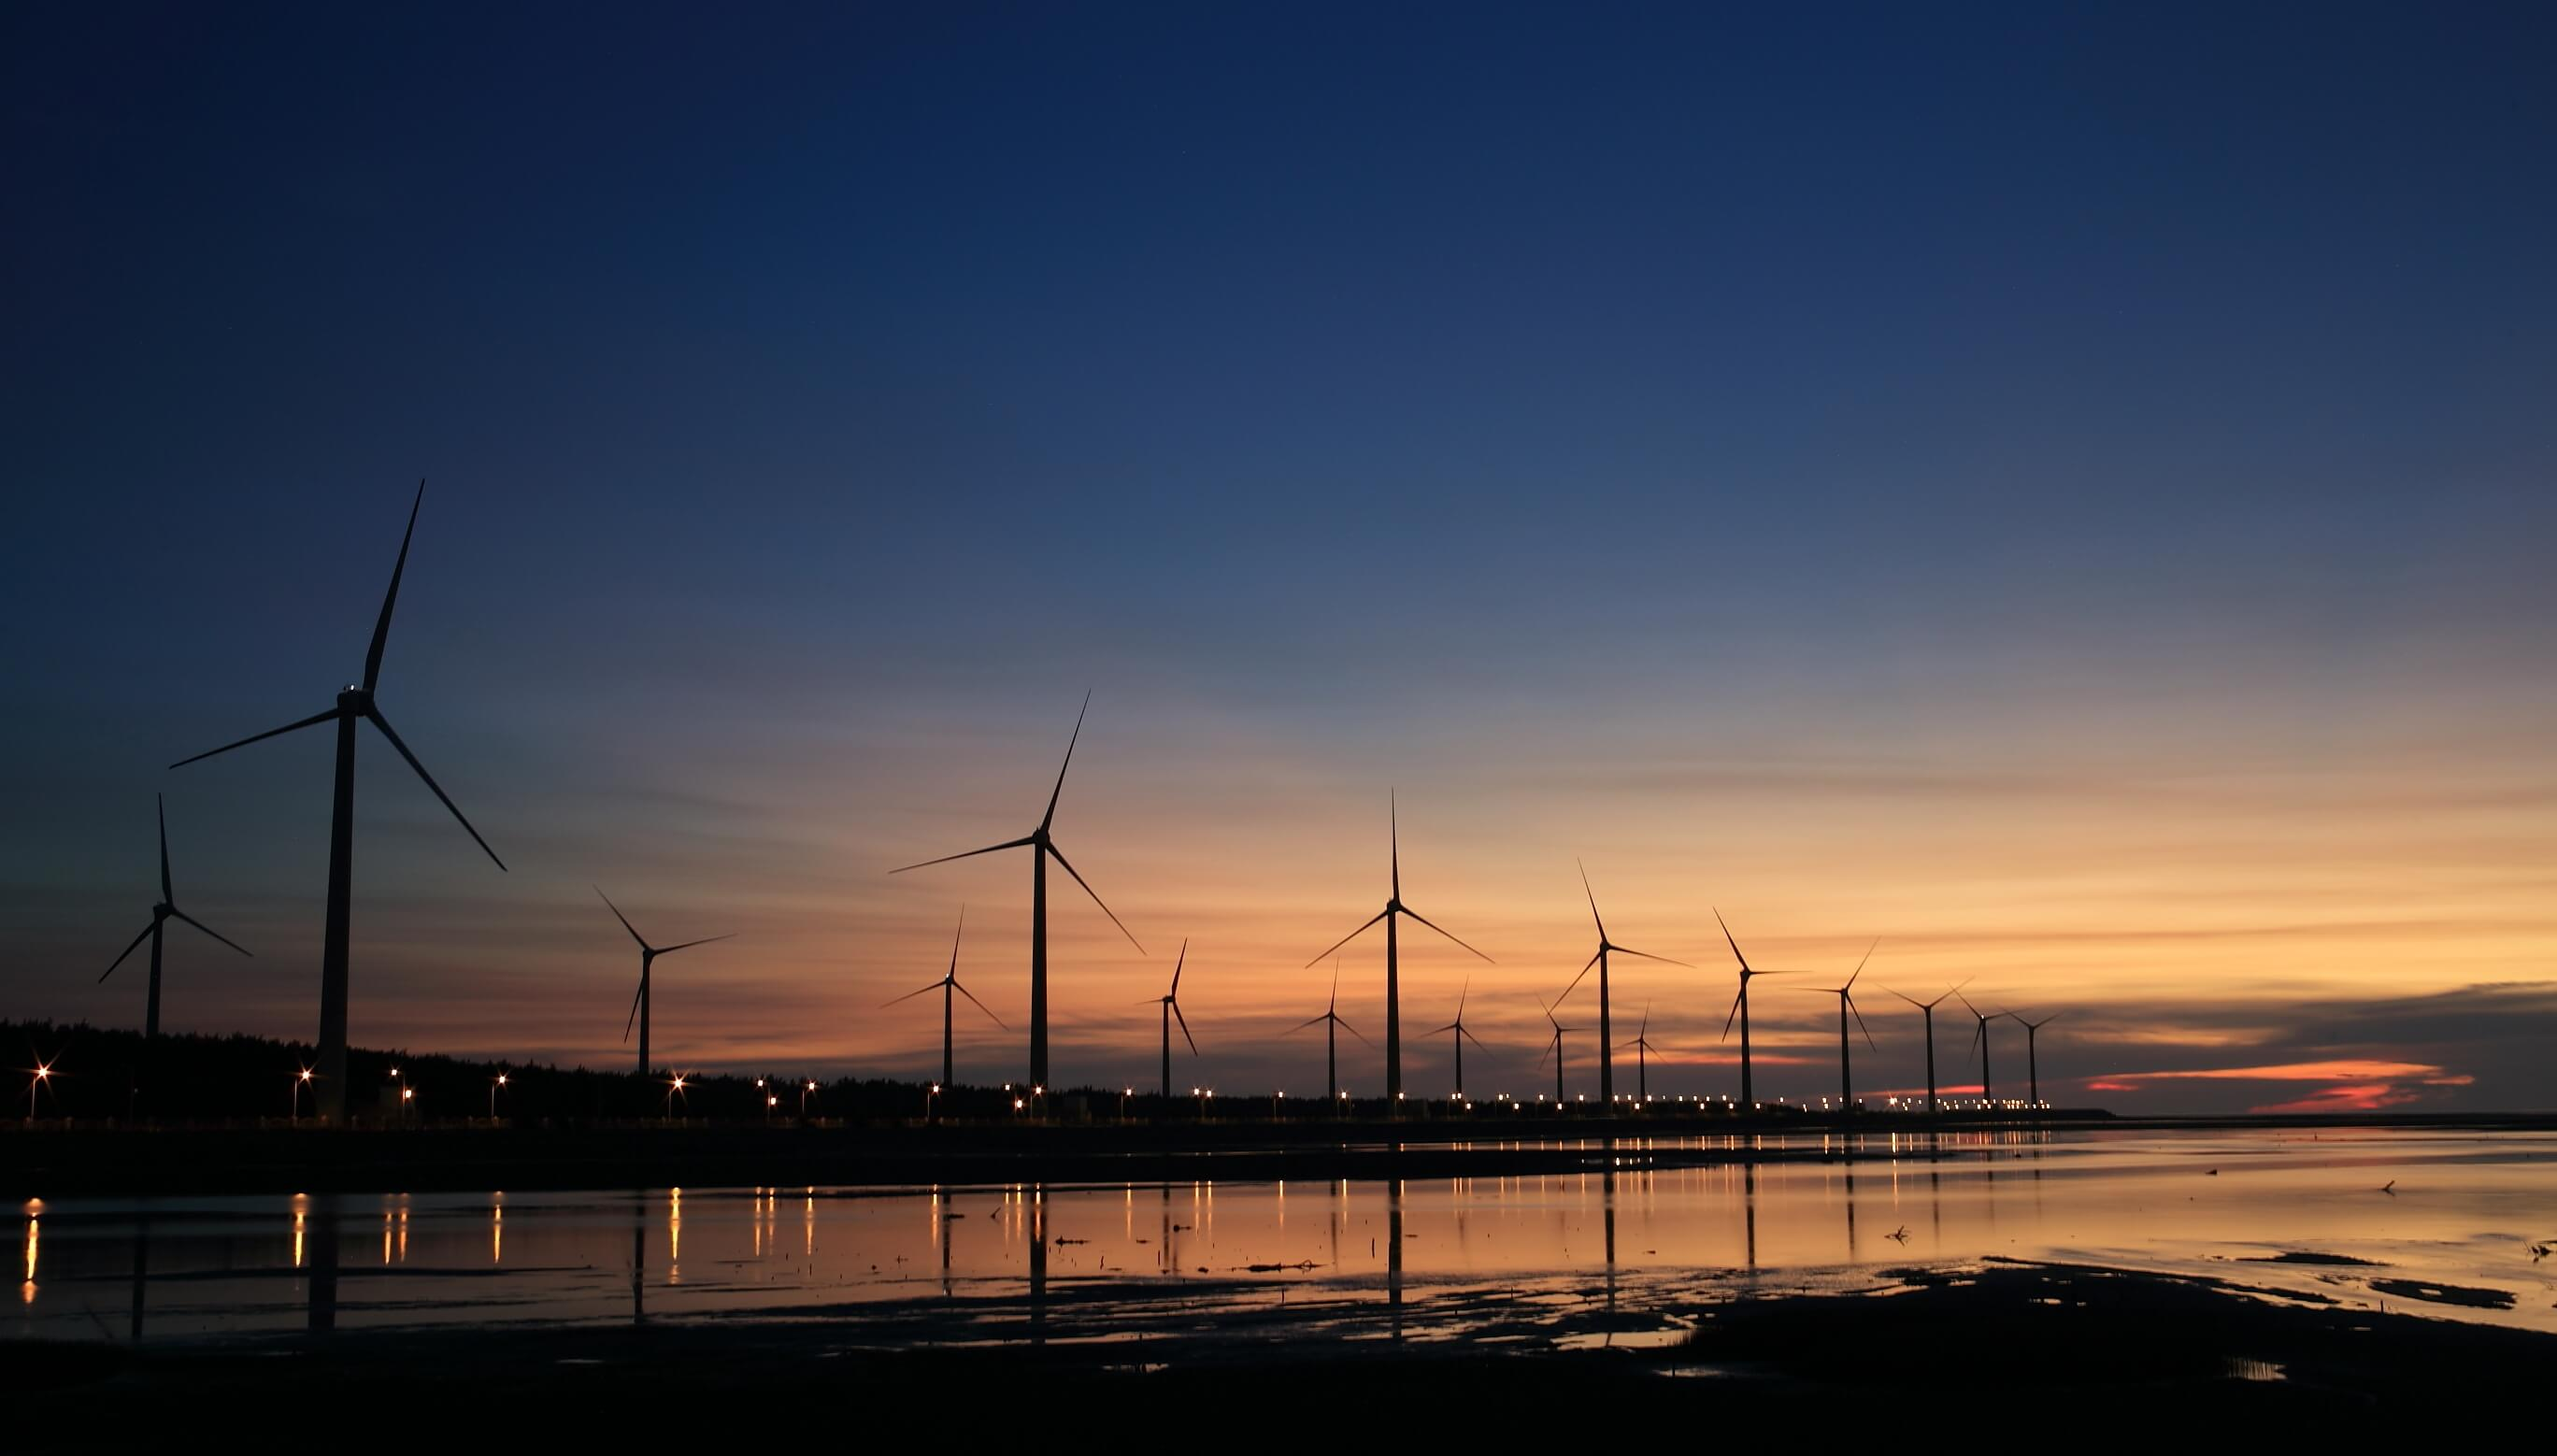
\includegraphics[height=5cm]{wind-turbines}
  \caption{Exemplo de figura.}
  \label{fig:exemplo-1}
\end{figure}
\end{lstlisting}

\end{frame}

\begin{frame}
  \frametitle{Exemplo de Figura}
  \begin{figure}[!htp]
    \centering
    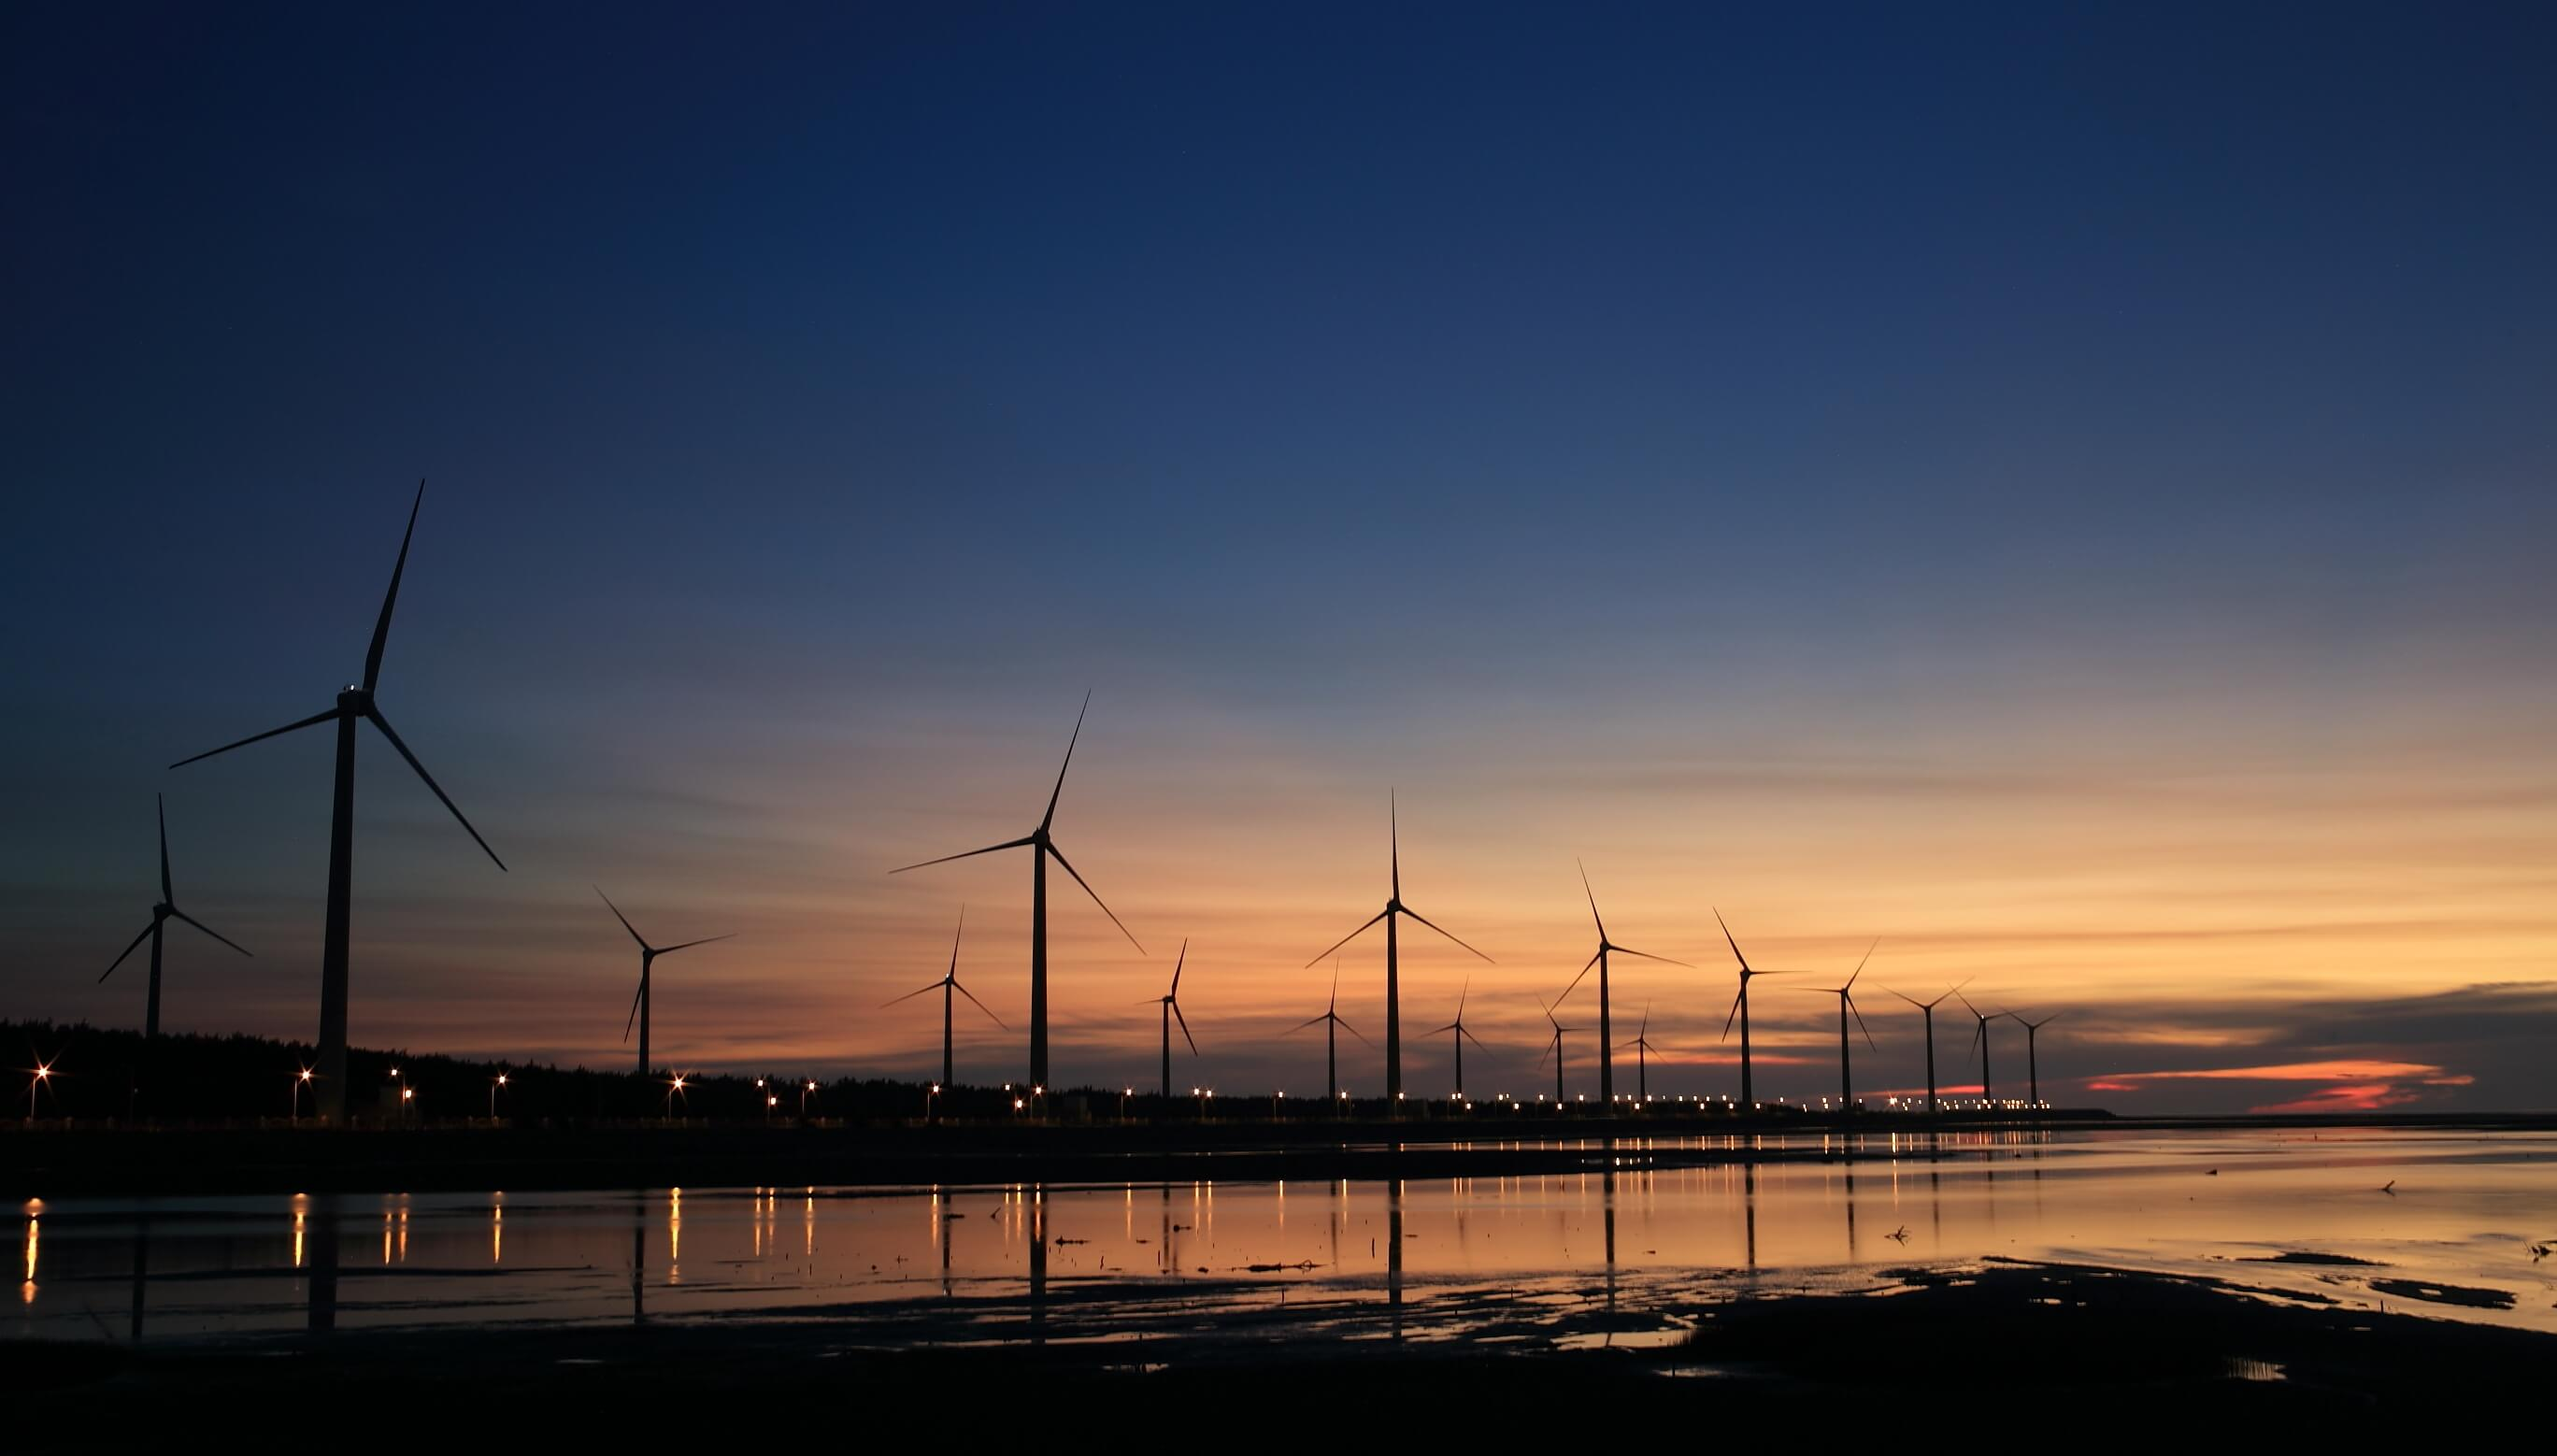
\includegraphics[height=6cm]{wind-turbines}
    \caption{Exemplo de figura.}
    \label{fig:exemplo-1}
  \end{figure}
  
\end{frame}


%% =============================================================================

\subsection{Tabelas}

%% =============================================================================


\begin{frame}[fragile]
  \frametitle{Inserindo Tabelas}

  Para inserir tabelas utilize o seguinte comando:

\begin{lstlisting}
\begin{table}[!htp]
  \centering
  \begin{tabular}{c c c}
    \hline\hline
    \textbf{Coluna 1} & \textbf{Coluna 2} & \textbf{Coluna 3} \\
    \hline\hline
    Item 1.1 & Item 1.2 & Item 1.3 \\ \hline
    ... 
    Item 5.1 & Item 5.2 & Item 5.3 \\
    \hline\hline
  \end{tabular}
  \caption{Exemplo de tabela.}
  \label{tab:exemplo-1}
\end{table}
\end{lstlisting}

\end{frame}

\begin{frame}[fragile]
  \frametitle{Exemplo de tabela}
  
  
  \begin{table}[!htp]
    \centering
    \begin{tabular}{c c c}
      \hline\hline
      \textbf{Coluna 1} & \textbf{Coluna 2} & \textbf{Coluna 3} \\
      \hline\hline
      Item 1.1 & Item 1.2 & Item 1.3 \\ \hline
      Item 2.1 & Item 2.2 & Item 2.3 \\ \hline
      Item 3.1 & Item 3.2 & Item 3.3 \\ \hline
      Item 4.1 & Item 4.2 & Item 4.3 \\ \hline
      Item 5.1 & Item 5.2 & Item 5.3 \\
      \hline\hline
    \end{tabular}
    \caption{Exemplo de tabela.}
    \label{tab:exemplo-1}
  \end{table}

  Para alterar o espaçamento entre as linhas, use o seguinte comando: \lstinline|\renewcommand*{\arraystretch}{1.25}|, no inicio do arquivo tex.

\end{frame}

\section[Outra Seção]{Outra Seção da Apresentação}

\begin{frame}[fragile]
  \frametitle{Referências Cruzadas}

  Para referênciar figuras e tabelas basta utilizar o comando:
  \lstinline|\ref{fig:exemplo-1}| é um exemplo de como referênciar a figura com
  \lstinline|\label{fig:exemplo-1}|.

  A Figura~\ref{fig:exemplo-1} mostra ...
  
\end{frame}



\end{document}

